\usetikzlibrary{calc}


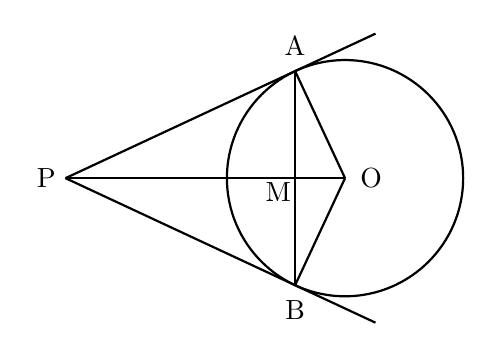
\begin{tikzpicture}[scale=1]

    % Define the center of the circle
    \coordinate (O) at (0,0);

    % Define points A and B on the circle
    % Angle 115 and 245 degrees closely match the proportions of the tangents in the image
    \coordinate (A) at (115:1.5);
    \coordinate (B) at (245:1.5);

    % Define point P on the x-axis where the two tangents intersect
    % For radius R=1.5 and angle 115 deg, x_P = -1.5 / cos(180-115) = -3.55
    \coordinate (P) at (-3.55, 0);

    % Define the intersection point M of chord AB and line PO
    \coordinate (M) at (-0.634, 0);

    % Draw the circle
    \draw[thick] (O) circle (1.5);

    % Draw the extended tangent lines from P through A and B
    % Using the calc library to extend the line beyond the tangent points
    \draw[thick] (P) -- ($(P)!1.35!(A)$);
    \draw[thick] (P) -- ($(P)!1.35!(B)$);

    % Draw the internal lines and segments
    \draw[thick] (P) -- (O); % Line segment PO
    \draw[thick] (A) -- (B); % Chord AB
    \draw[thick] (O) -- (A); % Radius OA
    \draw[thick] (O) -- (B); % Radius OB

    % Add labels to all points exactly as they appear
    \node[left] at (P) {P};
    \node[above, yshift=2pt] at (A) {A};
    \node[below, yshift=-2pt] at (B) {B};
    \node[right, xshift=2pt] at (O) {O};
    
    % Label M is positioned to the bottom-left of the intersection
    \node[below left, xshift=2pt, yshift=2pt] at (M) {M};

\end{tikzpicture}